\documentclass[10pt,a4paper]{article}

\usepackage[utf8]{inputenc}
\usepackage[T5]{fontenc}
\usepackage{amsmath, amssymb, amsfonts}
\usepackage[a4paper, top=14mm, bottom=14mm, left=16mm, right=16mm]{geometry}
\usepackage{graphicx}
\usepackage{xcolor}
\usepackage{booktabs, tabularx, array}
\usepackage{colortbl}
\usepackage{float}
\usepackage{fancyhdr}
\usepackage{enumitem}
\usepackage[unicode, colorlinks=true, linkcolor=primary, citecolor=secondary, urlcolor=secondary]{hyperref}

\emergencystretch=3em
\tolerance=2000
\hbadness=10000
\hfuzz=2pt
\setlength{\parskip}{3pt}
\setlength{\parindent}{0pt}

\definecolor{primary}{RGB}{0, 45, 98}
\definecolor{secondary}{RGB}{0, 102, 153}
\definecolor{tablehead}{RGB}{228, 238, 250}

\makeatletter
\renewcommand{\section}{\@startsection{section}{1}{\z@}%
  {-1.6ex \@plus -0.4ex \@minus -.2ex}%
  {0.6ex \@plus .1ex}%
  {\normalfont\normalsize\bfseries\color{primary}}}
\renewcommand{\subsection}{\@startsection{subsection}{2}{\z@}%
  {-1.2ex\@plus -0.3ex \@minus -.1ex}%
  {0.4ex \@plus .1ex}%
  {\normalfont\small\bfseries\color{secondary}}}
\makeatother

\setlength{\headheight}{13pt}
\pagestyle{fancy}
\fancyhf{}
\fancyhead[L]{\footnotesize\textit{ĐHQGHN - Trường Đại học Công nghệ (UET)}}
\fancyhead[R]{\footnotesize\textit{Bài thực hành số 8: Biểu cảm Khuôn mặt \& TurtleBot 4}}
\fancyfoot[C]{\footnotesize Trang \thepage}
\renewcommand{\headrulewidth}{0.4pt}

\renewcommand{\figurename}{Hình}
\renewcommand{\tablename}{Bảng}
\newcolumntype{Y}{>{\centering\arraybackslash}X}
\newcolumntype{R}{>{\raggedright\arraybackslash}X}

\begin{document}

\begin{center}
  {\large\bfseries\color{primary} BÁO CÁO KỸ THUẬT: BÀI THỰC HÀNH SỐ 8}\\[2pt]
  {\large\bfseries\color{primary} NHẬN DIỆN BIỂU CẢM KHUÔN MẶT BẰNG AI (DEEPFACE + OPENCV) VÀ ĐIỀU KHIỂN TURTLEBOT 4}\\[4pt]
  {\footnotesize \textbf{Họ và tên:} Nguyễn Quang Tuân \quad|\quad \textbf{MSSV:} 23020767 \quad|\quad \textbf{GVHD:} PGS.TS. Hoàng Văn Xiêm, CN. Nguyễn Quốc Bảo}\\
  {\footnotesize \textbf{Nền tảng:} ROS 2 Humble, Gazebo Fortress, RViz2, DeepFace \& OpenCV \quad|\quad \textbf{GitHub:} \url{https://github.com/Tuan404cl/Turtlebot_sim_test5}}\\
  {\footnotesize \textbf{Video Demo (Google Drive Public):} \href{https://drive.google.com/drive/folders/1vl4O0C9A4C3Ed_HwHmJAeVCzwEQZulCx?usp=drive_link}{drive.google.com/drive/folders/1vl4O0C9A4C3Ed\_HwHmJAeVCzwEQZulCx}}
\end{center}
\vspace{-4pt}
\noindent\rule{\textwidth}{0.6pt}

\section*{I. KIẾN TRÚC HỆ THỐNG VÀ LUỒNG XỬ LÝ ROS 2}
Hệ thống được thiết kế thành hai node ROS 2 độc lập kết nối với môi trường mô phỏng Gazebo Fortress và RViz2:
\begin{itemize}[leftmargin=14pt, itemsep=1pt, topsep=2pt]
  \item \textbf{Node nhận diện cảm xúc (\texttt{emotion\_recognition\_node.py}):} Đọc khung hình thời gian thực \texttt{640x480} từ Webcam (\texttt{/dev/video0}) hoặc từ bộ 06 ảnh khuôn mặt mẫu (\texttt{sample\_images\_dir}). Để duy trì tốc độ hiển thị giao diện OpenCV HUD mượt ($\sim 30\text{ FPS}$), node sử dụng cơ chế \textbf{1-slot latest-frame buffer} đưa ảnh sang luồng nền gọi \texttt{DeepFace.analyze(actions=['emotion'], detector\_backend='opencv')}. Điểm số 7 lớp FER-2013 được chuẩn hóa về đúng \textbf{06 biểu cảm mục tiêu} (\texttt{Happy}, \texttt{Sad}, \texttt{Neutral}, \texttt{Angry}, \texttt{Surprise}, \texttt{Fear}; gộp \texttt{disgust} vào \texttt{Neutral}) và đi qua bộ lọc \texttt{EmotionStabilizer} (trung bình trượt \texttt{smoothing\_window=4}, ngưỡng \texttt{min\_confidence=0.30}, khử rung \texttt{debounce\_frames=2}, và watchdog mất mặt \texttt{face\_lost\_timeout\_sec=1.5s}) trước khi xuất lên topic \texttt{/detected\_emotion}.
  \item \textbf{Node điều khiển quỹ đạo (\texttt{emotion\_control\_node.py}):} Subscribe \texttt{/detected\_emotion}, \texttt{/odom}, \texttt{/scan} và phát vận tốc \texttt{geometry\_msgs/msg/Twist} lên \texttt{/cmd\_vel} ở tần số \texttt{20 Hz}. Node tự động cấu hình tham số \texttt{safety\_override='full'} trên dịch vụ \texttt{/motion\_control/set\_parameters} của đế iRobot Create 3 để mở khóa chuyển động lùi (\texttt{Angry}), giám sát vật cản LiDAR trước/sau ($\ge 0.25\text{ m}$) và tự động phanh dừng khi mất tín hiệu quá $1.5\text{ s}$.
\end{itemize}

\section*{II. BẢNG ÁNH XẠ 06 BIỂU CẢM KHUÔN MẶT VÀ QUỸ ĐẠO ĐIỀU KHIỂN TURTLEBOT 4}

\begin{table}[H]
\centering
\footnotesize
\renewcommand{\arraystretch}{1.18}
\begin{tabularx}{\textwidth}{|c|l|c|l|c|c|R|}
\hline
\rowcolor{tablehead}
\textbf{TT} & \textbf{Biểu cảm} & \textbf{Nhãn ROS 2} & \textbf{Hành động của TurtleBot} & \textbf{$v$ (m/s)} & \textbf{$\omega$ (rad/s)} & \textbf{Cơ chế động học \& An toàn} \\
\hline
1 & \textbf{Happy} (Vui vẻ) & \texttt{Happy} & Quỹ đạo cong sang trái & $+0.18$ & $+0.55$ & Cung tròn trái $R = 0.327\text{ m}$, LiDAR trước $\ge 0.25\text{ m}$ \\
\hline
2 & \textbf{Sad} (Buồn) & \texttt{Sad} & Quỹ đạo cong sang phải & $+0.18$ & $-0.55$ & Cung tròn phải $R = 0.327\text{ m}$, LiDAR trước $\ge 0.25\text{ m}$ \\
\hline
3 & \textbf{Neutral} (Bình thường) & \texttt{Neutral} & Dừng tại chỗ & $0.00$ & $0.00$ & Dừng tức thời; hủy ngay xoay \texttt{Surprise} nếu đang chạy \\
\hline
4 & \textbf{Angry} (Tức giận) & \texttt{Angry} & Lùi nhẹ về phía sau & $-0.12$ & $0.00$ & Mở khóa Create 3 (\texttt{safety\_override} = \texttt{'full'}), LiDAR sau \\
\hline
5 & \textbf{Surprise} (Ngạc nhiên) & \texttt{Surprise} & Xoay một vòng tại chỗ & $0.00$ & $+1.00$ & Tích phân góc yaw từ \texttt{/odom} đủ $2\pi\text{ rad}$ ($360^\circ$) rồi dừng \\
\hline
6 & \textbf{Fear} (Sợ hãi) & \texttt{Fear} & Tiến nhẹ về phía trước & $+0.12$ & $0.00$ & Tiến thẳng tốc độ êm, bảo vệ LiDAR trước $\ge 0.25\text{ m}$ \\
\hline
\end{tabularx}
\caption{Bảng ánh xạ 06 trạng thái biểu cảm khuôn mặt sang lệnh vận tốc \texttt{/cmd\_vel} của TurtleBot 4.}
\end{table}

\section*{III. KẾT QUẢ THỰC NGHIỆM VÀ KIỂM THỬ TỰ ĐỘNG}

\begin{figure}[H]
  \centering
  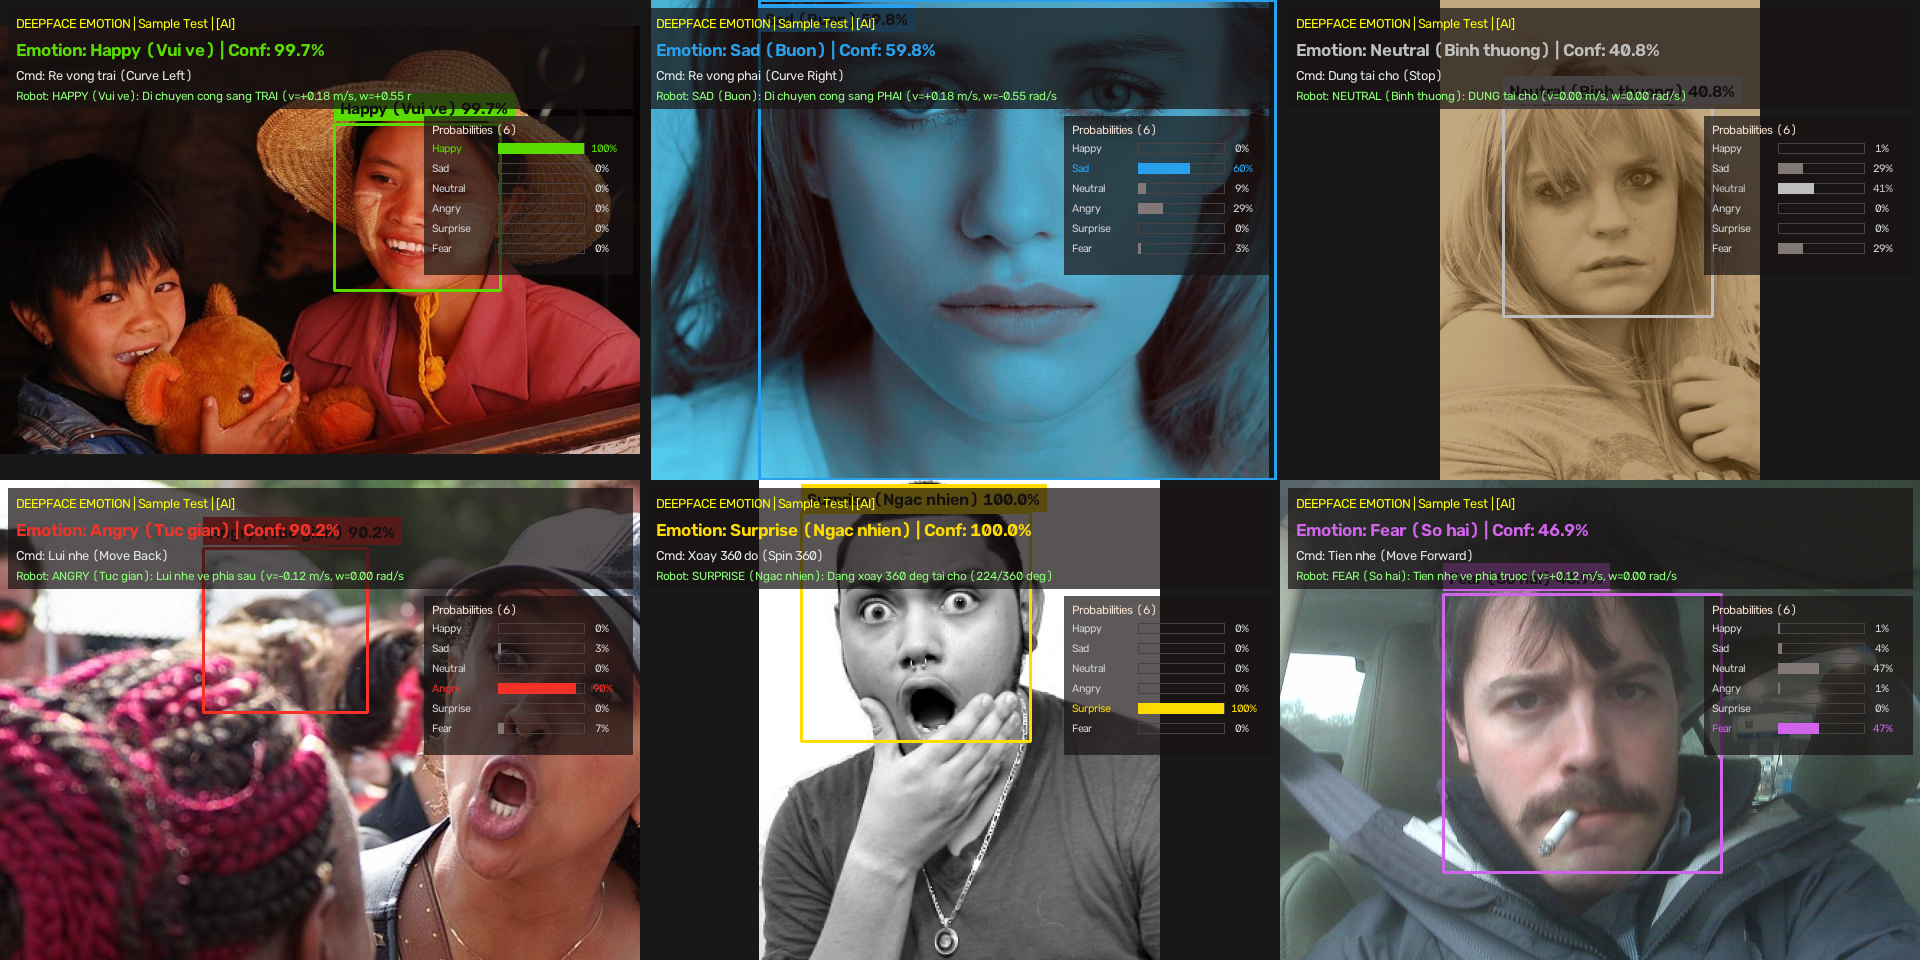
\includegraphics[width=0.96\textwidth]{figures/emotion_6_faces_grid.png}
  \caption{Kết quả nhận diện bằng DeepFace và giao diện HUD OpenCV (Bounding Box, độ tin cậy \%, biểu đồ 6 thanh xác suất và trạng thái lệnh điều khiển Robot) trên bộ ảnh khuôn mặt người thật.}
\end{figure}

\begin{figure}[H]
  \centering
  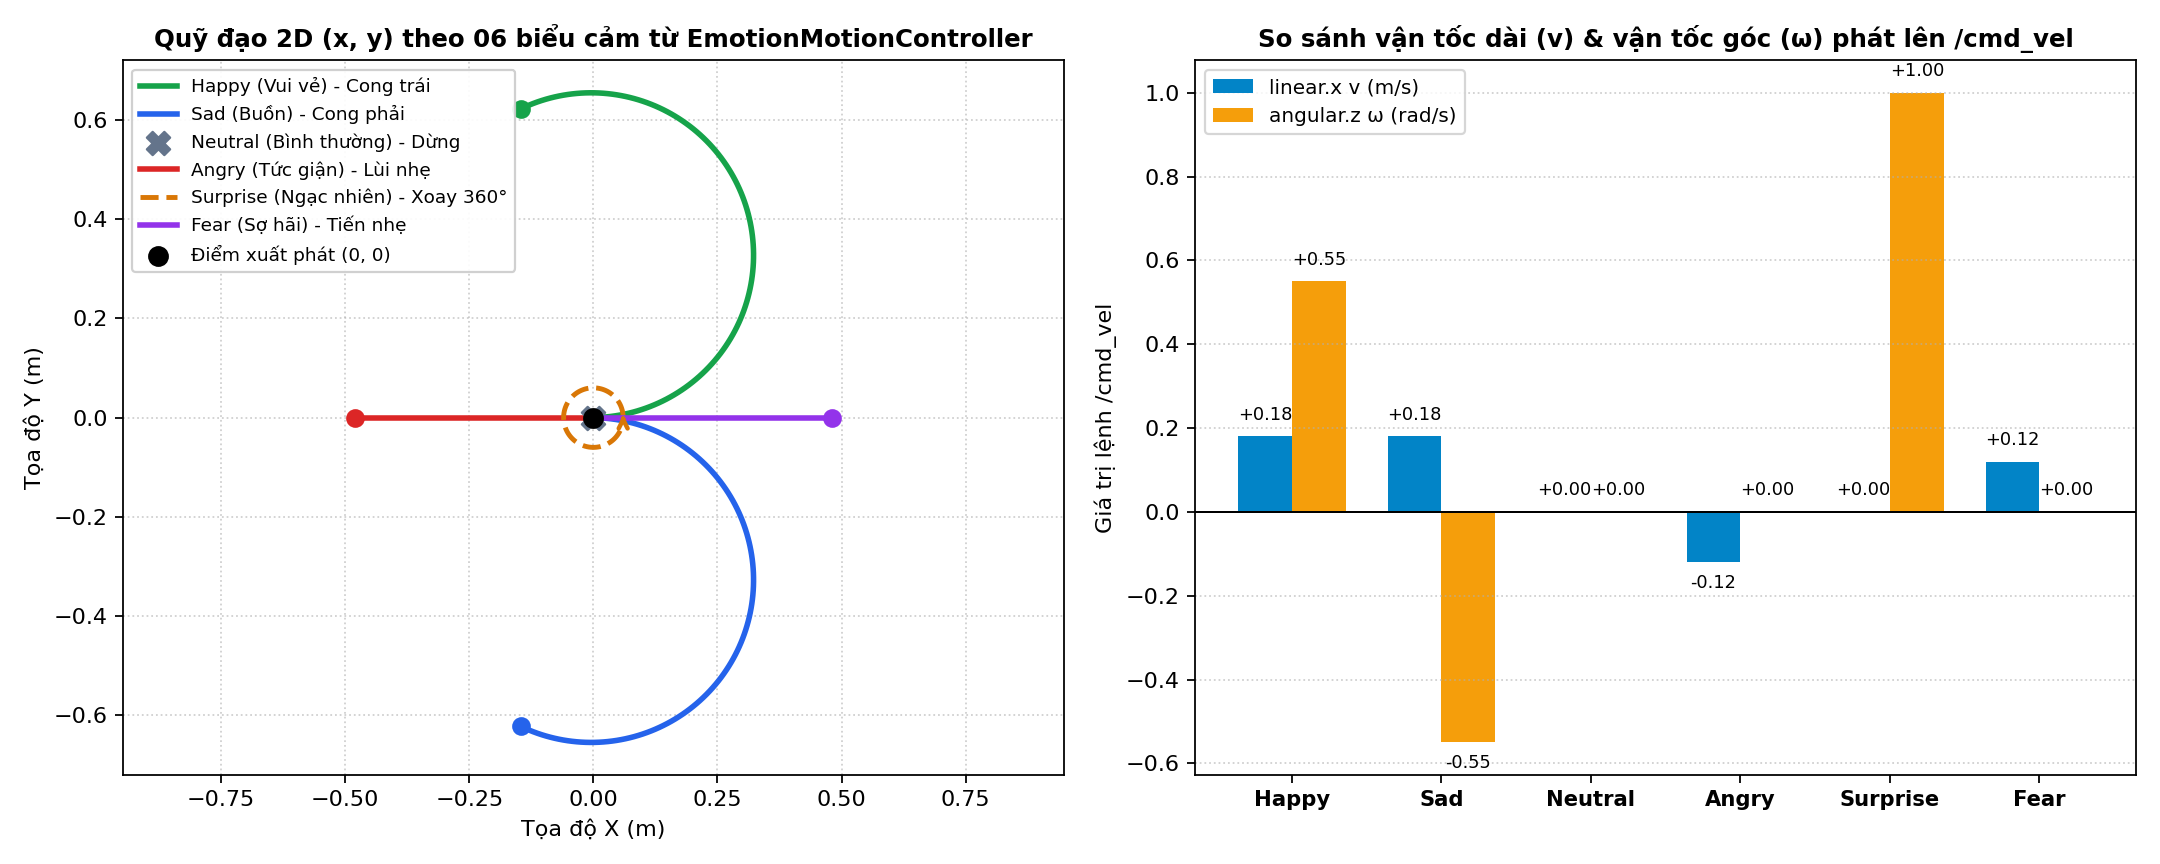
\includegraphics[width=0.96\textwidth]{figures/emotion_trajectories_odom.png}
  \caption{Quỹ đạo di chuyển 2D $(x, y)$ của TurtleBot 4 tương ứng với 06 biểu cảm (trái) và biểu đồ đối chiếu vận tốc dài $v$, vận tốc góc $\omega$ trên \texttt{/cmd\_vel} (phải).}
\end{figure}

\section*{IV. TRÌNH DIỄN THỰC TẾ TRONG GAZEBO FORTRESS, RVIZ2 VÀ TELEMETRY ROS 2}
Hệ thống được chạy trình diễn tích hợp trực tiếp trong thế giới \texttt{warehouse} của Gazebo Fortress (tự động \texttt{Auto Undock} và bật \texttt{safety\_override='full'}), đồng thời mở RViz2 (\texttt{map}, \texttt{/scan}, \texttt{AMCL}, \texttt{EmotionHUD}) và cửa sổ OpenCV DeepFace HUD qua chuỗi 06 ảnh khuôn mặt mẫu (\texttt{sample\_hold\_sec=8.5s}, \texttt{use\_sim\_time=false}):
\begin{itemize}[leftmargin=14pt, itemsep=1pt, topsep=2pt]
  \item \textbf{Video ghi hình thực tế:} \texttt{/home/tuan/Videos/emotion\_control\_demo.mp4} (\texttt{2560x1600}, H.264 \texttt{yuv420p}, \texttt{15 fps}, \texttt{1389} khung hình, thời lượng \texttt{92.60 s}, dung lượng \texttt{33,621,221 bytes} / \texttt{32.06 MiB}); bản công khai tại \href{https://drive.google.com/drive/folders/1vl4O0C9A4C3Ed_HwHmJAeVCzwEQZulCx?usp=drive_link}{Google Drive}.
  \item \textbf{Quỹ đạo \& An toàn đo từ \texttt{demo\_telemetry.json} (\texttt{951} mẫu @ \texttt{10 Hz}, \texttt{94.25 s}):} Xuất phát tại $(-1.105, -0.149)\text{ m}$, kết thúc tại $(1.156, -0.575)\text{ m}$; tổng quãng đường \texttt{/odom} đạt $7.050\text{ m}$ (dịch chuyển ròng $2.301\text{ m}$). Chu kỳ 1 hoàn toàn không va chạm; sang Chu kỳ 2 (\texttt{Sad}), phanh an toàn LiDAR phía trước kích hoạt đúng tại $0.2289\text{ m} < 0.25\text{ m}$ (\texttt{rear\_min = 0.3403 m}). Độ tin cậy AI trung bình đạt $75.96\%$ trên $857$ bản tin (\texttt{/cmd\_vel = 1,883}, \texttt{/odom = 4,948}, \texttt{/scan = 4,988}).
\end{itemize}

\begin{figure}[H]
  \centering
  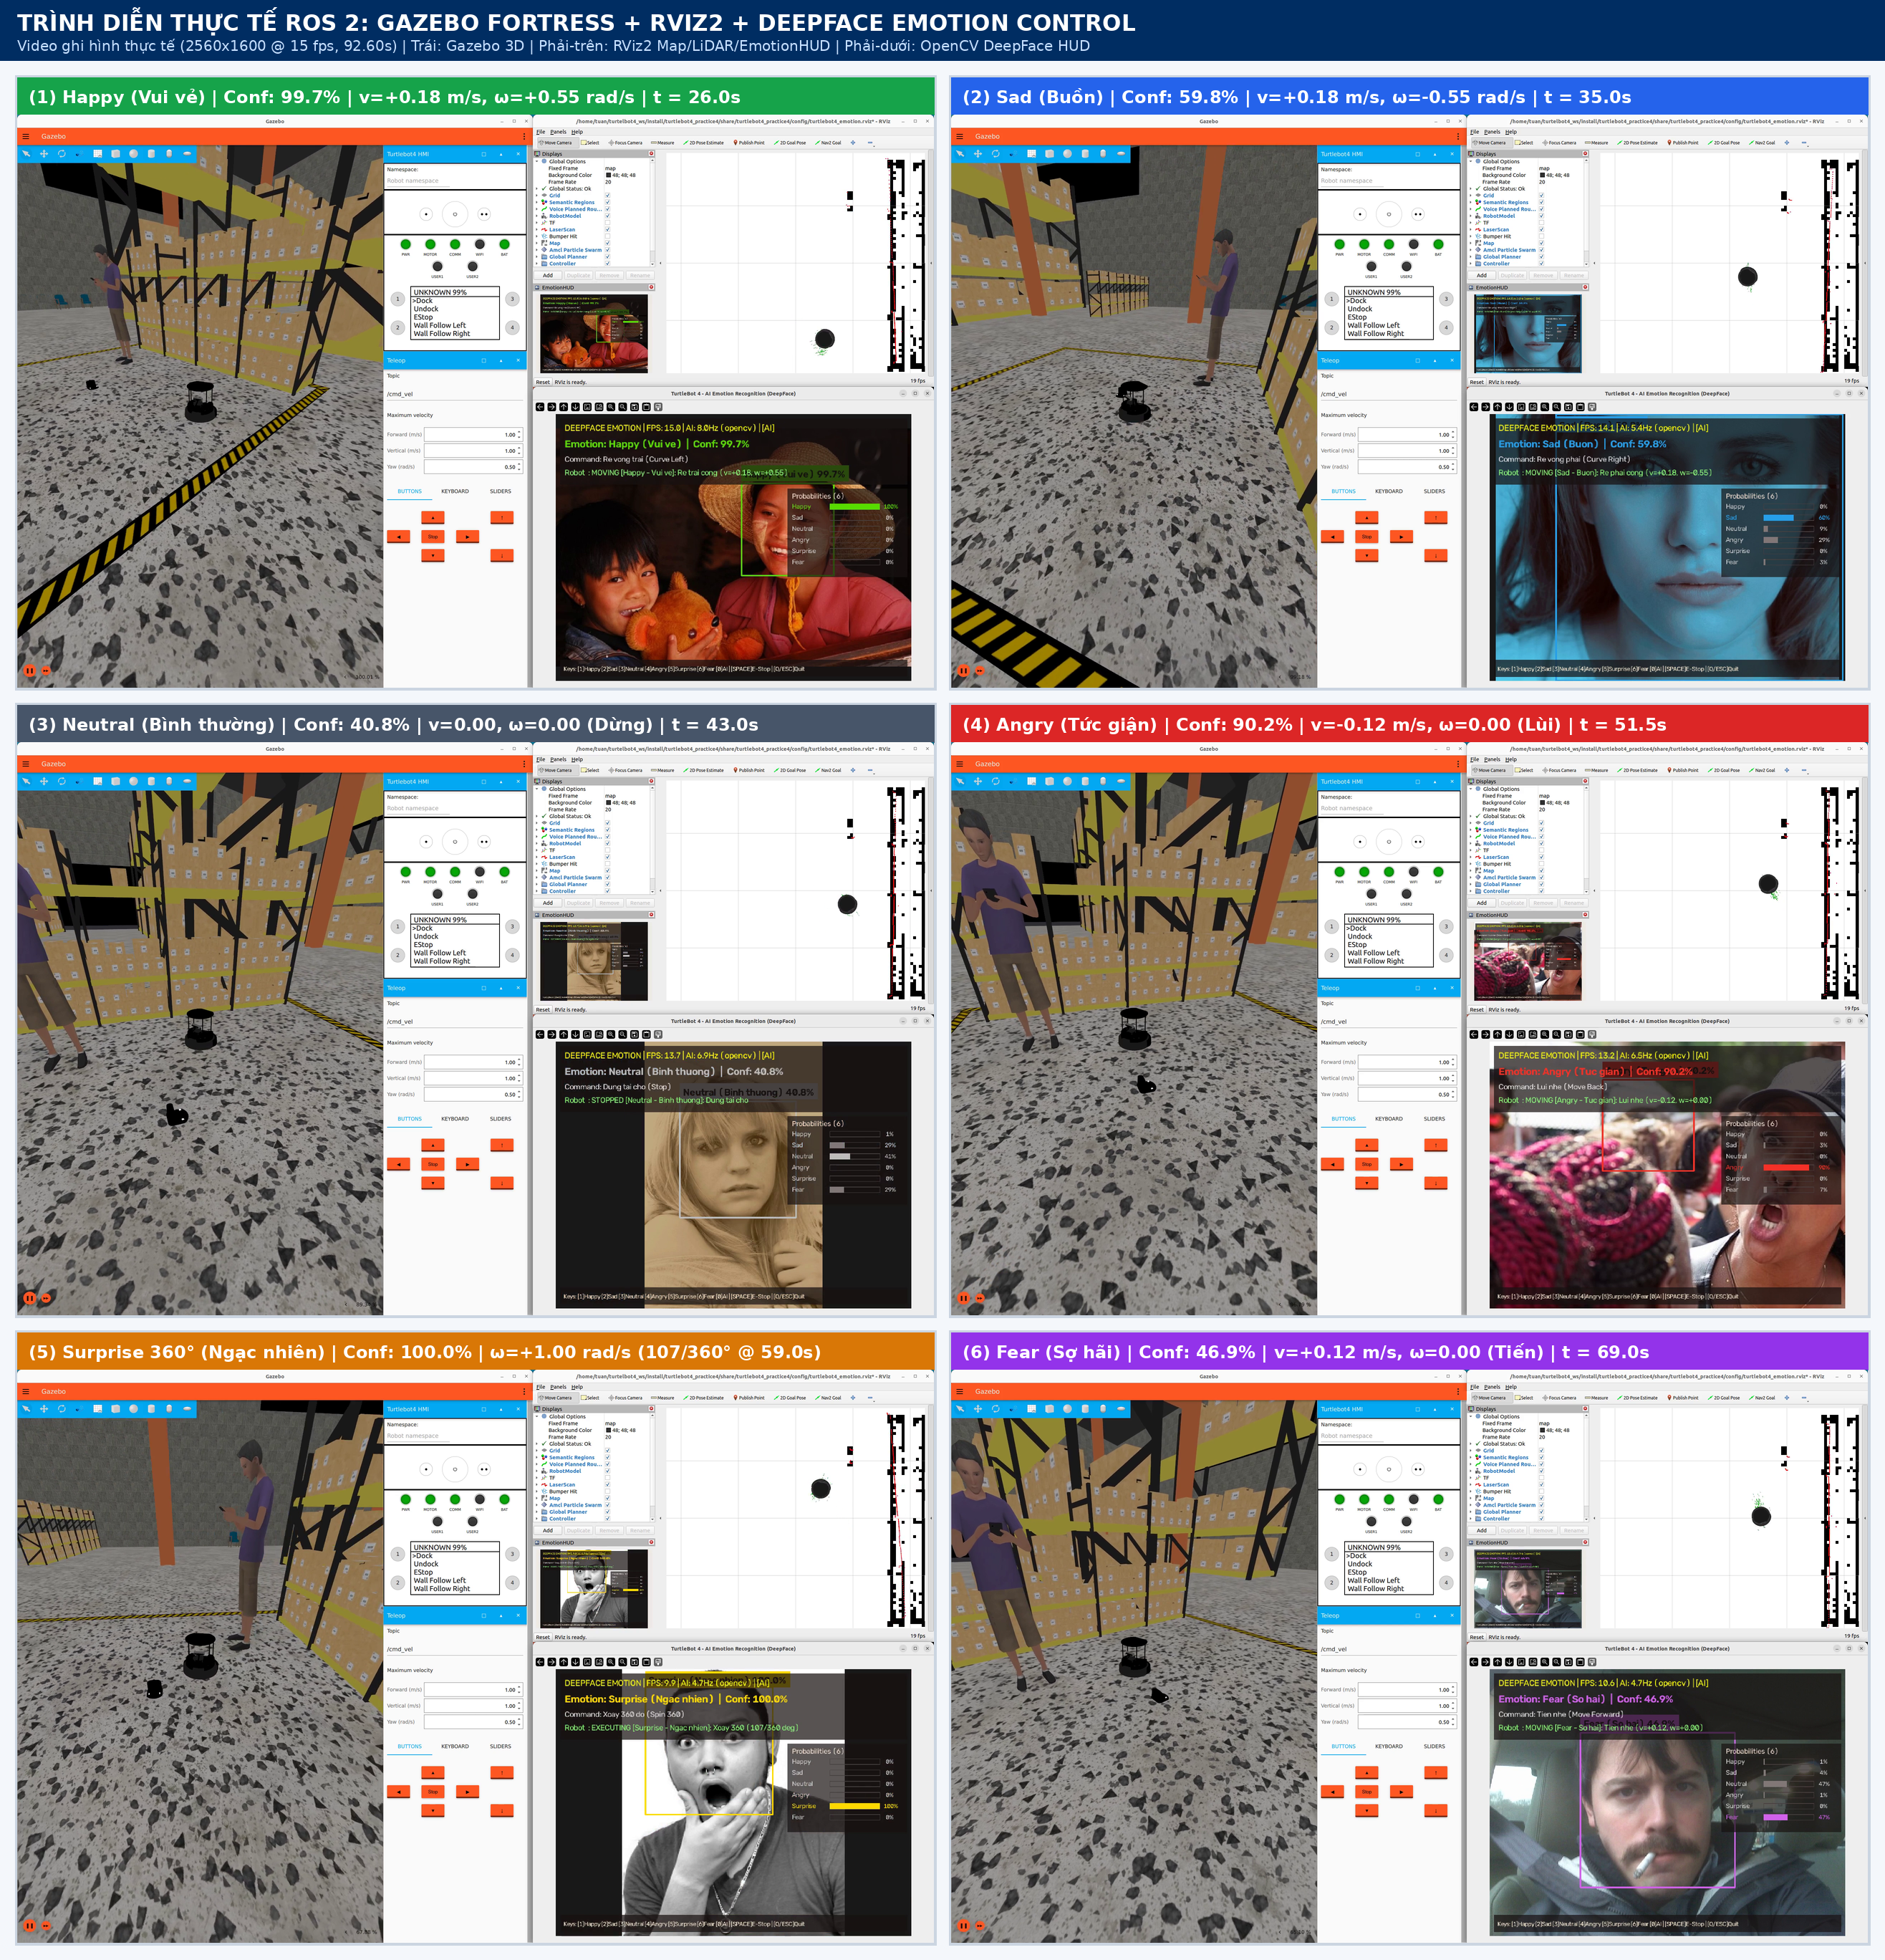
\includegraphics[width=0.98\textwidth,height=0.78\textheight,keepaspectratio]{figures/emotion_live_demo_composite.png}
  \caption{Ảnh tổng hợp 6 khung hình từ video \texttt{/home/tuan/Videos/emotion\_control\_demo.mp4} cho 06 biểu cảm (\texttt{Happy @ 26.0s}, \texttt{Sad @ 35.0s}, \texttt{Neutral @ 43.0s}, \texttt{Angry @ 51.5s}, \texttt{Surprise @ 59.0s}, \texttt{Fear @ 69.0s}), hiển thị đồng thời Gazebo 3D, RViz2 và OpenCV DeepFace HUD.}
\end{figure}

\begin{figure}[H]
  \centering
  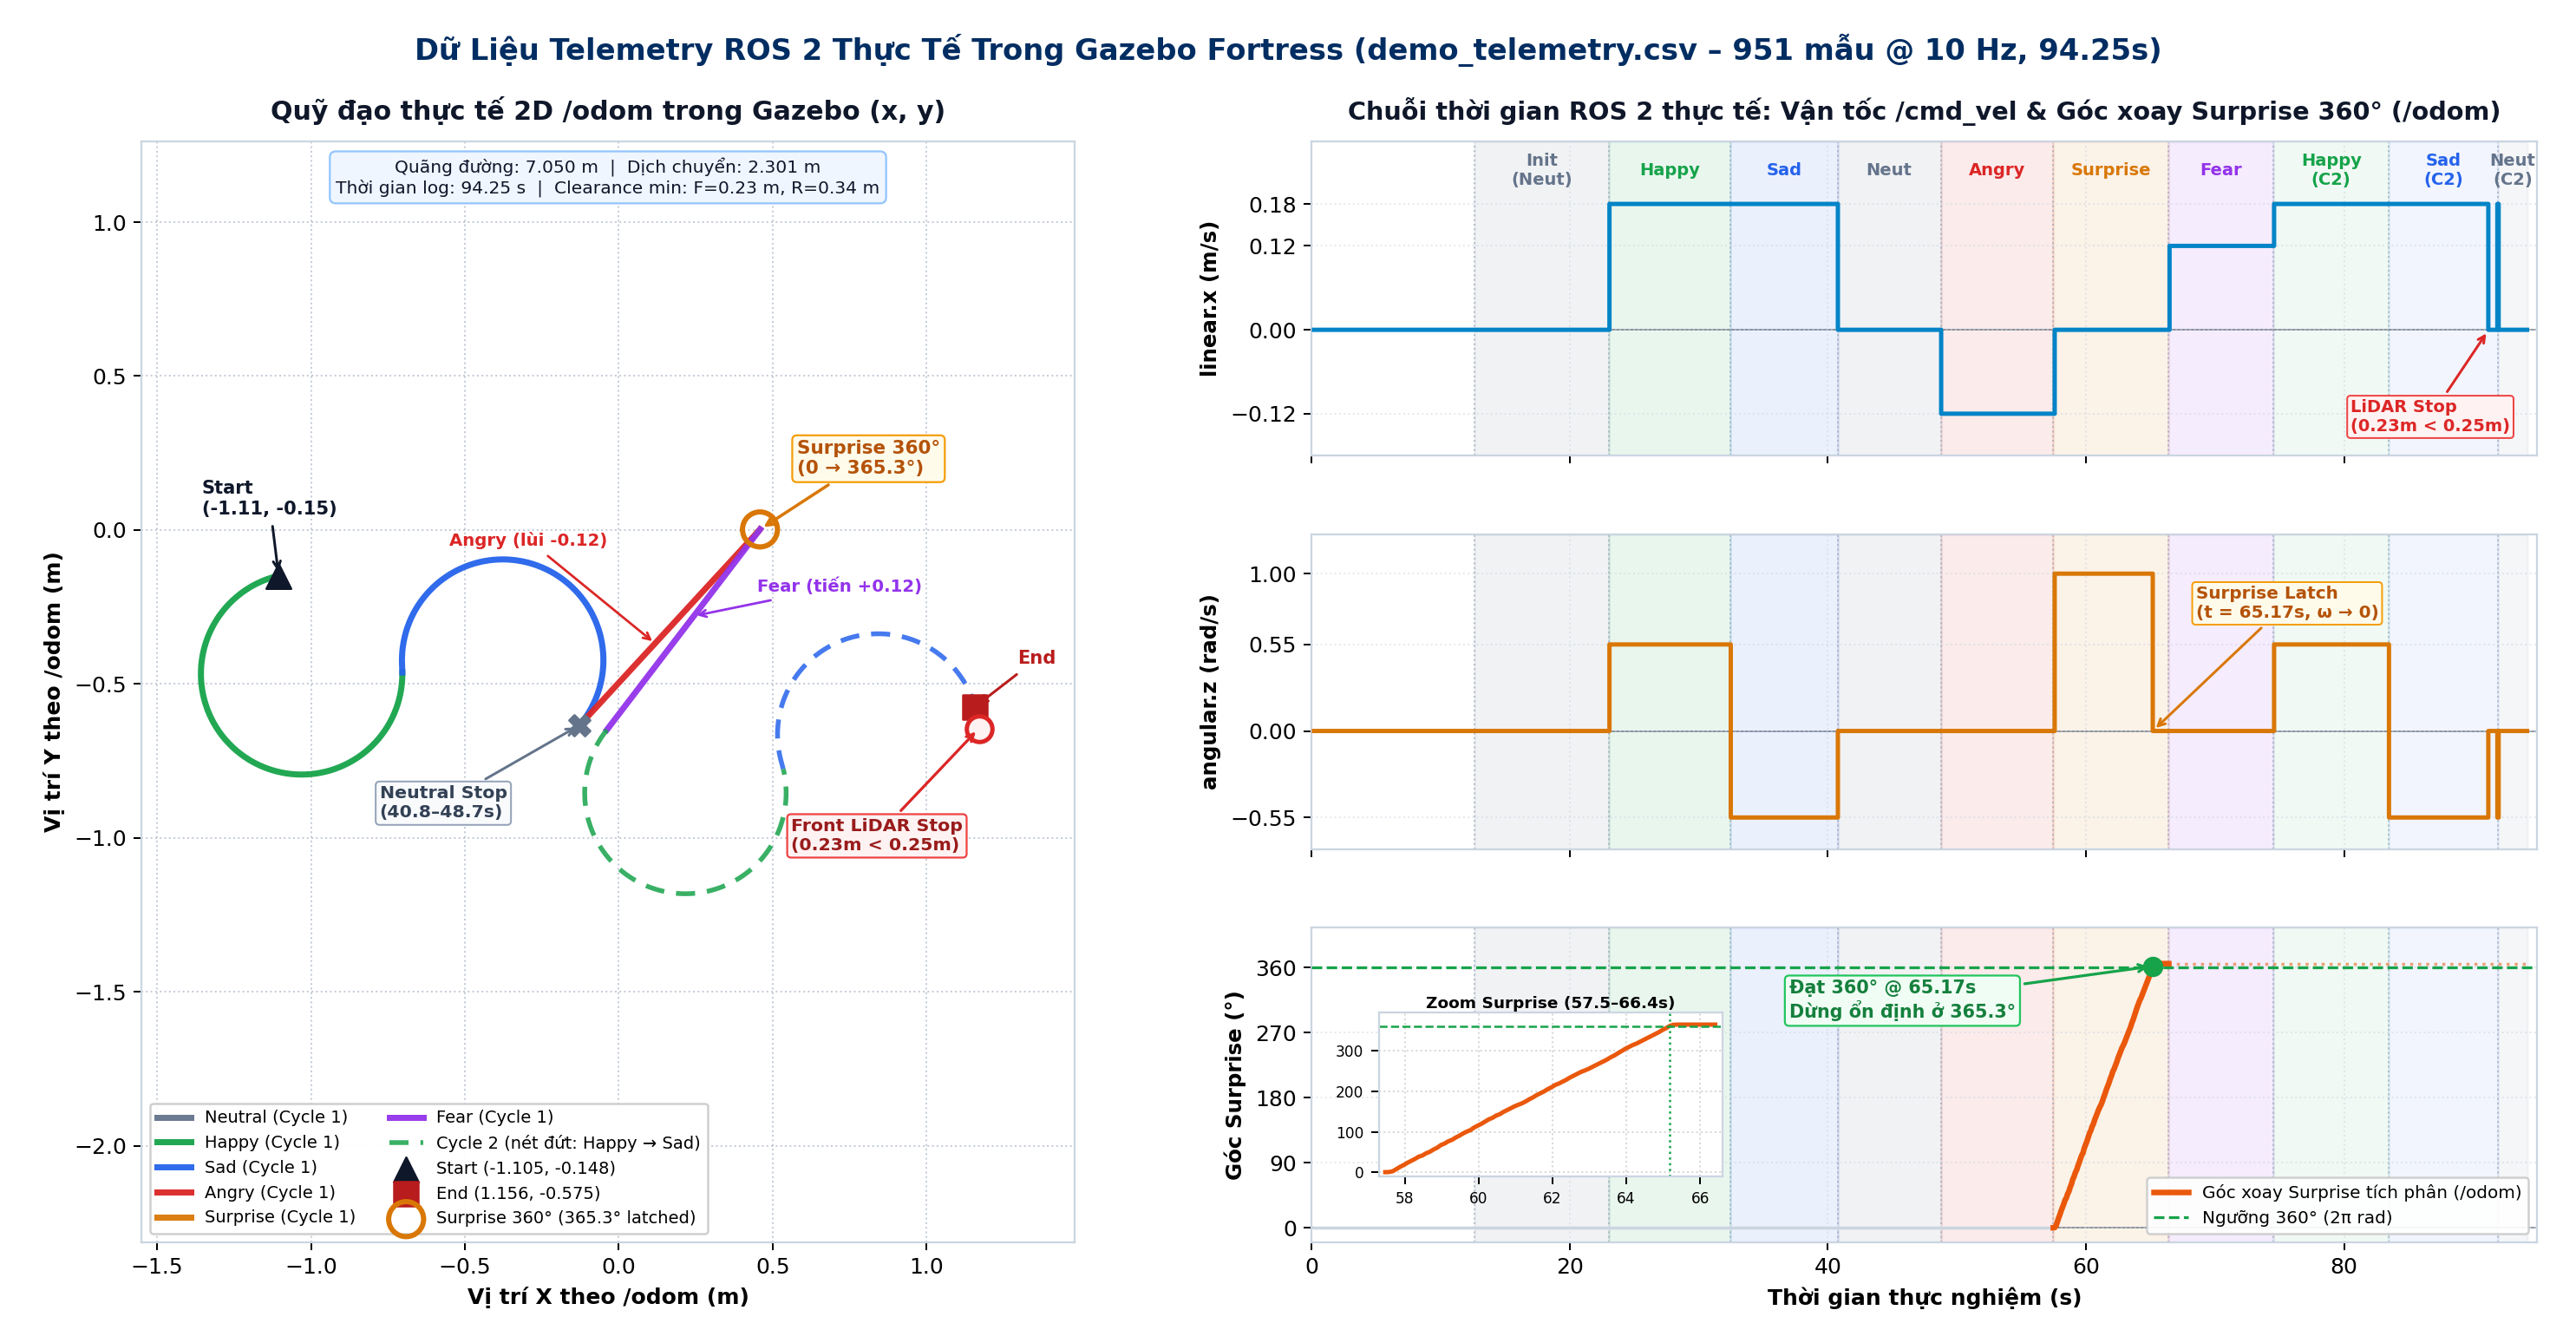
\includegraphics[width=0.98\textwidth]{figures/emotion_live_odom_telemetry.png}
  \caption{Dữ liệu telemetry ROS 2 thực tế từ \texttt{demo\_telemetry.csv}: quỹ đạo 2D \texttt{/odom} (trái) và chuỗi thời gian \texttt{linear.x}, \texttt{angular.z}, góc xoay \texttt{Surprise} tích phân $0 \rightarrow 365.3^\circ$ khóa chốt dừng ở $360^\circ$ (phải).}
\end{figure}

\begin{table}[H]
\centering
\footnotesize
\renewcommand{\arraystretch}{1.15}
\begin{tabularx}{\textwidth}{|l|c|c|c|c|c|R|}
\hline
\rowcolor{tablehead}
\textbf{Biểu cảm} & \textbf{Mẫu} & \textbf{TG (s)} & \textbf{Mean $v_x$ (Peak)} & \textbf{Mean $\omega_z$ (Peak)} & \textbf{AI Conf} & \textbf{Diễn biến đo thực tế trong Gazebo} \\
\hline
\texttt{Neutral} & 207 & 20.6634 & $0.0000$ ($0.00$) & $0.0000$ ($0.00$) & $69.78\%$ & Khởi tạo ($12.65\text{--}23.01\text{s}$), C1 ($40.75\text{--}48.74\text{s}$), C2 cuối \\
\hline
\texttt{Happy} & 183 & 18.3336 & $+0.1800$ ($0.18$) & $+0.5500$ ($0.55$) & $96.34\%$ & C1 ($23.01\text{--}32.43\text{s}$) + C2 ($74.54\text{--}83.45\text{s}$), cong trái $R=0.327\text{ m}$ \\
\hline
\texttt{Sad} & 168 & 16.8041 & $+0.1725$ ($0.18$) & $-0.5271$ ($0.55$) & $58.35\%$ & C1 ($32.43\text{--}40.75\text{s}$) + C2 ($83.45\text{--}91.94\text{s}$), phanh LiDAR ở $0.23\text{ m}$ \\
\hline
\texttt{Angry} & 87 & 8.7224 & $-0.1200$ ($0.12$) & $0.0000$ ($0.00$) & $88.58\%$ & C1 ($48.74\text{--}57.47\text{s}$), lùi thẳng với \texttt{safety\_override='full'} \\
\hline
\texttt{Surprise} & 90 & 8.9403 & $-0.0013$ ($0.12$) & $+0.8444$ ($1.00$) & $96.67\%$ & C1 ($57.47\text{--}66.41\text{s}$), xoay đủ $365.261^\circ$ rồi latch dừng tại $360^\circ$ \\
\hline
\texttt{Fear} & 81 & 8.1356 & $+0.1200$ ($0.12$) & $0.0000$ ($0.00$) & $46.34\%$ & C1 ($66.41\text{--}74.54\text{s}$), tiến thẳng êm về phía trước ($+0.12\text{ m/s}$) \\
\hline
\end{tabularx}
\caption{Bảng tổng hợp thông số telemetry ROS 2 thực tế theo từng trạng thái biểu cảm (\texttt{demo\_telemetry.json}).}
\end{table}

\textbf{Kết quả kiểm thử tự động (\texttt{pytest}):} Toàn bộ 41/41 kịch bản kiểm thử trong \texttt{test/test\_emotion\_control.py} (chuẩn hóa nhãn, lọc nhiễu \texttt{EmotionStabilizer}, 6 vector \texttt{Twist}, tích phân góc xoay $360^\circ$ qua biên $\pm\pi$, hủy lệnh bằng \texttt{Neutral}, Watchdog và LiDAR safety) đều đạt \textbf{41 PASSED (100\%)} trong $4.90\text{ s}$.

\section*{V. HƯỚNG DẪN CHẠY CHƯƠNG TRÌNH}
\begin{itemize}[leftmargin=14pt, itemsep=2pt, topsep=2pt]
  \item \textbf{Chạy tích hợp đầy đủ (Gazebo + RViz2 + Auto Undock + Webcam AI):}\\
  {\footnotesize\texttt{./src/turtlebot4\_practice4/scripts/run\_emotion\_control.sh}}
  \item \textbf{Chạy trình diễn tự động với bộ 06 ảnh khuôn mặt mẫu:}\\
  {\footnotesize\texttt{./src/turtlebot4\_practice4/scripts/run\_emotion\_control.sh \textbackslash}\\
  \texttt{\quad sample\_images\_dir:=/home/tuan/turtelbot4\_ws/src/turtlebot4\_practice4/config/emotion\_samples \textbackslash}\\
  \texttt{\quad sample\_hold\_sec:=8.5}}
  \item \textbf{Chỉ chạy 2 node AI \& Điều khiển:}\\
  {\footnotesize\texttt{./src/turtlebot4\_practice4/scripts/run\_emotion\_control.sh launch\_sim:=false}}
\end{itemize}

\end{document}
